
%---------------
%----SECTION----
%---------------
% \newpage
\section{Our model: Diffusion-based VampPrior VAE} \label{sec:proposed_approach}
In this work, we introduce the Diffusion-based VampPrior VAE (DVP-VAE). It is a deep hierarchical VAE model that approximates the optimal prior distribution at all levels of the hierarchical VAE in an efficient way.

\subsection{VampPrior for hierarchical VAE}
Directly using the VampPrior approximation (see Eq.~\ref{eq:vamp_prior_approx}) for deep hierarchical VAE can be very computationally expensive since it requires evaluating the variational posterior of all latent variables for $K$ pseudoinputs at each training iteration. Thus, \citet{tomczak2018vae} proposed a modification in which only the top latent variable uses VampPrior, namely:
\begin{equation}\label{eq:hierarchical_vamp}
\begin{aligned}
p^*(\rvz_{1:L}) &= \mathbb{E}_{\rvx} q_{\phi, \theta}(\rvz_{1:L}|\rvx) \\
&\approx \mathbb{E}_{\rvx} q_{\phi, \theta}(\rvz_{L}|\rvx) p_{\theta}(\rvz_{1:L-1})  \\
&\approx \mathbb{E}_{r(\rvu)} q_{\phi, \theta}(\rvz_{L}|\rvu) p_{\theta}(\rvz_{1:L-1}),
\end{aligned}
\end{equation}
where $r(\rvu) = \frac1K \sum_k \delta(\rvu - \rvu_k)$ with learnable pseudoinputs $\{u_k\}_{k=1}^K$.
In this approach, there are a few problems: (i) how to pick the \textit{best} number of pseudoinputs $K$, (ii) how to train pseudoinputs, and (iii) how to train the VampPrior in a scalable fashion. The last issue results from the first two problems and the fact that the dimensionality of pseudoinputs is the same as the original data, i.e., $\mathrm{dim}(\rvu) = \mathrm{dim}(\rvx)$.

Here, we propose a different prior parameterization to overcome all these three problems. Our approach consists of three steps in which we approximate the VampPrior at all levels of the deep hierarchical VAE. 
We propose to \textit{amortize} the distribution of pseudoinputs in VampPrior and use them to \textit{directly} condition the prior distribution:
\begin{equation}\label{eq:our_vamp_prior}
p^*(\rvz_{1:L}) = \mathbb{E}_{\rvx} q_{\phi, \theta}(\rvz_{1:L}|\rvx) \approx \mathbb{E}_{\rvx, r(\rvu|\rvx)} p_{\theta}(\rvz_{1:L}|\rvu),
\end{equation}
where we use $r(\rvu) = \mathbb{E}_{\rvx}[r(\rvu | \rvx)]$. Using $r(\rvu | \rvx)$, which is cheap to evaluate for any input, we avoid the expensive procedure of encoding pseudoinputs along with the inputs $\rvx$. Amortizing the VampPrior solves the problem of picking $K$ and helps with training pseudoinputs. 

To define conditional distribution, we treat pseudoinputs $\rvu$ as a result of some noisy non-trainable transformation of the input datapoints $\rvx$. 
Let us consider a transformation $f: \mathcal{X}^{D} \rightarrow \mathcal{X}^{P}$, i.e., $\rvu = f(\rvx) + \sigma \varepsilon $, where $\varepsilon$ is a standard Gaussian random variable and $\sigma$ is the standard deviation. Note that by applying $f$, e.g., a linear transformation, we can lower the dimensionality of pseudoinputs, $\mathrm{dim}(\rvu) < \mathrm{dim}(\rvx)$, resulting in better scalability. As a result, we get the following amortized distribution:
\begin{equation}\label{eq:amortized_vampprior_posterior}
    r(\rvu|\rvx) = \mathcal{N}(\rvu | f(\rvx), \sigma^2 I).
\end{equation}
The crucial part then is how to choose the transformation $f$. It is a non-trivial choice since we require the following properties of $f$: (i) it should result in $\mathrm{dim}(\rvu) < \mathrm{dim}(\rvx)$, (ii) $\rvu$ should be a \textit{reasonable} representation of $\rvx$, (iii) it should be \textit{easily} computable (e.g., fast for scalability). We have two candidates for such transformations. First, we can consider a downsampled version of an image. Second, we propose to use a discrete cosine transform. We will discuss this approach in the following subsection.

Moreover, the outlined amortized VampPrior in the previous two steps seems to be a good candidate for efficient and scalable training. However, it does not seem to be suitable for generating new data. Therefore, we propose including pseudoinputs as the final level in our model and use a marginal distribution $\hat{r}(\rvu)$ that approximates $r(\rvu)$. Here, we propose to use a diffusion-based model for $\hat{r}(\rvu)$.


\subsection{DCT-based pseudoinputs}

The first important component in our approach is the form of the non-trainable transformation from the input to the pseudoinput space. We assume that for $\rvu$ to be a \textit{reasonable} representation of $\rvx$ means that $\rvu$ should preserve general patterns (information) of $\rvx$, but it does not necessarily contain any high-frequency details of $\rvx$. To achieve this, we propose to use a \textit{discrete cosine transform}\footnote{We consider the most widely used type-II DCT.} (DCT) to convert the input into a frequency domain and then filter the high-frequency component. 

\paragraph{DCT} DCT~\citep{ahmed1974discrete} is a widely used transformation in signal processing for image, video, and audio data. For example, it is part of the JPEG standard \citep{pennebaker1992jpeg}. 
For instance, consider a signal as a $3$-dimensional tensor $\rvx \in \mathbb{R}^{\text{c} \times D \times D}$. DCT is a linear transformation that decomposes each channel $\rvx_{i}$ on a basis consisting of cosine functions of different frequencies: $\rvu_{DCT, i} = \rmC \rvx_{i} \rmC^{\top}$, where for all pairs $(k=0,n)$: $\rmC_{k,n} = \sqrt{\frac{1}{D}}$,  and for all pairs $(k,n)$ such that $k>0$: $\rmC_{k,n} = \sqrt{\frac{2}{D}} \cos \left(\frac{\pi}{D}\left(n+\frac{1}{2}\right) k\right)$. 
 

% \begin{table}[t]
% \begin{minipage}[t]{0.45\textwidth}
\begin{algorithm}[t] %[!htbp]
\caption{$f_{\text{dct}}$: Create DCT-based pseudoinputs}
\label{alg:context_forward}
\begin{algorithmic}
 \\\hrulefill
        \State \hskip-3mm \textbf{Input}: $\rvx \in \mathbb{R}^{\text{c} \times D \times D}, \rmS\in \mathbb{R}^{c \times d \times d}, d \in \mathbb{R}$
    \State $\rvu_{\text{DCT}} = \text{DCT}(\rvx)$
        \State $\rvu_{\text{DCT}} = \text{Crop}(\rvu_{\text{DCT}}, d)$ %\Comment{Keep $\text{Ch} \times d\times d$ (top-left).}
        \State $\rvu_{\text{DCT}} = \frac{\rvu_{\text{DCT}}}{\rmS} $  % \Comment{Normalize}
        \State  \hskip-3mm \textbf{Return}: $\rvu_{\text{DCT}}\in \mathbb{R}^{\text{c} \times d \times d}$
\end{algorithmic}
\end{algorithm}
% \end{minipage}\hfill
% \begin{minipage}[t]{0.49\textwidth}
\begin{algorithm}[t] %[!htbp]
\caption{$f^{\dagger}_{\text{dct}}$: Invert DCT-based pseudoinputs}
\label{alg:context_backward}
\begin{algorithmic} %[1]
 \\\hrulefill
        \State \hskip-3mm \textbf{Input}: $\rvu_{\text{DCT}} \in \mathbb{R}^{\text{c} \times d \times d}, \rmS \in \mathbb{R}^{\text{c} \times d \times d}, D$
        \State $\rvu_{\text{DCT}} = \rvu_{\text{DCT}} \cdot \rmS$
        \State $\rvu_{\text{DCT}} = \text{zero\_pad}(\rvu_{\text{DCT}}, D-d)$% \Comment{Pad to $\text{Ch} \times D\times D$.}
        \State $\rvu_{\text{x}} = \text{iDCT}(\rvu_{\text{DCT}})$ %\Comment{Apply inverse DCT}
        \State \hskip-3mm \textbf{Return}: $\rvu_{\text{x}} \in \mathbb{R}^{\text{c} \times D \times D}$
\end{algorithmic}
\end{algorithm}
% \end{minipage}
% \end{table}

\paragraph{Our transformation} We use the DCT transform as the first step in the procedure of computing pseudoinputs. 
Let us assume that each channel of $\rvx$ is $D\times D$. We select the desired size of the context $d < D$ and remove (crop) $D-d$ bottom rows and right-most columns for each channel in the frequency domain since they contain the highest-frequency information. 
Finally, we perform normalization using the matrix $\rmS$ that contains the maximal absolute value of each frequency. 
We calculate this matrix once (before training the model) using all the training data: $\rmS = \max_{\rvx \in \mathcal{D}_{\text{train}}} |\text{DCT}(\rvx)|$. 
% As a result, we get context variables whose values are in the range $[-1, 1]$. 
The complete procedure is described in Algorithm~\ref{alg:context_forward} and we denote it as $f_{\text{dct}}$. 

In the frequency domain, a pseudoinput has a smaller spatial dimension than its corresponding datapoint. This allows us to use a small prior model %(described in Section~\ref{subsection:diff_prior}) 
and lower the memory consumption.
However, we noticed empirically that conditioning the amortized VampPrior (see Eq.~\ref{eq:our_vamp_prior}) on the pseudoinput in the original domain makes training easier. Therefore, the pseudo-inverse is applied as a part of the TopDown path. First, we start by multiplying the pseudoinput by the normalization matrix $\rmS$. 
Afterward, we pad each channel with zeros to account for the "lost" high frequencies. 
Lastly, we apply the inverse of the Discrete Cosine Transform (iDCT). 
% We explain in more detail how $f_{\text{ctx}}$ and $f^{\dagger}_{\text{ctx}}$ are used in the model architecture in Section~\ref{subsec:arch_decode}.
We denote the procedure for converting a pseudoinput from the frequency domain to the data domain as $f^{\dagger}_{\text{dct}}$ and describe it in Algorithm~\ref{alg:context_backward}.


% We describe this procedure in Algorithm~\ref{alg:context_backward}.  
% We refer to our TopDown hierarchical VAE with a DCT-based context as DCT-VAE.


% Due to cropping operation, the context computation is no longer invertible. 
% However, we can still go back from frequency to data domain. 


\subsection{Our Ladder VAE and Training Objective}
% Consider the context random variable $\rvu$ to be determined by a non-learnable transformation $f(\cdot)$ of the input $\rvx$.
% , namely, $\rvu \sim q(\rvu| f(\rvx))$. 

We use the TopDown architecture and extend this model with a deterministic, non-trainable function to create the pseudoinput. In our generative model, pseudoinputs are treated as another set of latent variables:
\begin{align}
    p_{\theta}(\rvx, \rvz_{1:L}, \rvu) &= p_{\theta}(\rvx| \rvz_{1:L})p_{\theta}(\rvz_{1:L}|\rvu)r(\rvu), \\
    p_{\theta}(\rvz_{1:L}|\rvu) &= p_{\theta}(\rvz_L |\rvu) \prod_{l=1}^{L-1} p_{\theta}(\rvz_l |\rvz_{l+1:L},  \rvu).
\end{align}
Then, we choose variational posteriors in which pseudoinput latent variables are conditionally independent with all other latent variables given the datapoint $\rvx$, that is:
\begin{align}
    q_{\phi}(\rvz_{1:L}, \rvu| \rvx) &= q_{\phi}(\rvz_{1:L}| \rvx)r(\rvu| \rvx),  \\
    q_{\phi}(\rvz_{1:L}| \rvx)  & = q_{\phi}(\rvz_L |\rvx) \prod_{l=1}^{L-1} q_{\phi}(\rvz_l |\rvz_{l+1:L},  \rvx),\\
    r(\rvu| \rvx) & = \mathcal{N}(\rvu | f(\rvx), \sigma^2 I).
\end{align}
In the variational posteriors, we use the amortization of $r(\rvu)$ outlined in Eq.~\ref{eq:our_vamp_prior}.

\begin{figure}[t]
% \begin{wrapfigure}{r}{0.55\textwidth}
\centering
\subfloat[Ladder VAE \label{subfig:ladder_graph}]{%\subfigure{
    \begin{tikzpicture}[node distance=.4cm]
  % ENCODER: ALL RV
  \node[obs, minimum size=0.75cm] (X) {$\rvx$};
  \node[latent, minimum size=0.75cm, above=0.2cm of X] (z1) {$\rvz_1$};
  \node[latent, minimum size=0.75cm, above=0.4cm of z1] (z2) {$\rvz_2$};
  \node[latent, minimum size=0.75cm, above=0.4cm of z2] (z3) {$\rvz_3$};
  % \node[latent, minimum size=0.75cm, above=0.4cm of z3] (zL) {$\rvu$};
  % \node[inner sep=0,minimum size=0.5cm, left=0.2cm of X] (k1) {}; % invisible node
  \node[inner sep=0,minimum size=0.5cm, right=0.1cm of X] (k2) {}; % invisible node
  \node[inner sep=0,minimum size=0.5cm, left=0.05cm of z3] (k3) {}; % invisible node
  % ENCODER:ALL ARROWS 
  % \draw[-Latex, dashed, black] (X) -- (k1.center) |- node[above]{} (zL);
  \draw[-Latex, black] (X) -- (k2.center) |- node[above]{} (z3);
  \draw[-Latex, black] (X) -- (k2.center) |- node[above]{} (z2);
  \draw[-Latex, black] (X) -- (k2.center) |- node[above]{} (z1);
  \draw[-Latex, black!10!blue] (z3) -- (k3.center) |- node[above]{} (z1);
  \edge[-Latex, black!10!blue] {z3} {z2};
  \edge[-Latex, black!10!blue] {z2} {z1};
  \end{tikzpicture}
  \quad
  \begin{tikzpicture}[node distance=.4cm]
   \node[obs, minimum size=0.75cm] (X_gen) {$\rvx$};
  \node[latent, minimum size=0.75cm, above=0.2cm of X_gen] (z1_gen) {$\rvz_1$};
  \node[latent, minimum size=0.75cm, above=0.4cm of z1_gen] (z2_gen) {$\rvz_2$};
  \node[latent, minimum size=0.75cm, above=0.4cm of z2_gen] (z3_gen) {$\rvz_3$};
  
    \node[inner sep=0,minimum size=0.5cm, left=0.05cm of z3_gen] (k4) {}; % invisible node

    \node[inner sep=0,minimum size=0.5cm, right=0.05cm of z3_gen] (k5) {}; % invisible node
    \node[inner sep=0,minimum size=0.5cm, right=0.05cm of z2_gen] (k6) {}; % invisible node
    \node[inner sep=0,minimum size=0.5cm, right=0.05cm of z1_gen] (k7) {}; % invisible node
    
    % \node[inner sep=0,minimum size=0.5cm, left=0.2cm of zL_gen] (k8) {}; % invisible node
    
    % shared path
    \edge[-Latex, black!10!blue] {z3_gen} {z2_gen};
    \edge[-Latex, black!10!blue] {z2_gen} {z1_gen};
    \draw[-Latex, black!10!blue] (z3_gen) -- (k4.center) |- node[above]{} (z1_gen);

    % conditional likelihood
    \draw[-Latex, black] (z3_gen) -- (k5.center) |- (X_gen);
    \draw[-Latex, black] (z2_gen) -- (k6.center) |- (X_gen);
    \draw[-Latex, black] (z1_gen) -- (k7.center) |- (X_gen);

    % context
    % \draw[-Latex, black] (zL_gen) -- (k8.center) |- ($(z1_gen.west)+(0.1em,-0.8em)$);
    % \draw[-Latex, black] (zL_gen) -- (k8.center) |- ($(z2_gen.west)+(0.1em,-0.8em)$);
    % \draw[-Latex, black] (zL_gen) -- (k8.center) |- ($(z3_gen.west)+(0.1em,-0.8em)$);
\end{tikzpicture}}
% \hfill
\hskip 40pt
\subfloat[Ladder VAE with pseudoinouts
 \label{subfig:ctx_ladder_graph}]{
     \begin{tikzpicture}[node distance=.4cm]
  % ENCODER: ALL RV
  \node[obs, minimum size=0.75cm] (X) {$\rvx$};
  \node[latent, minimum size=0.75cm, above=0.2cm of X] (z1) {$\rvz_1$};
  \node[latent, minimum size=0.75cm, above=0.4cm of z1] (z2) {$\rvz_2$};
  \node[latent, minimum size=0.75cm, above=0.4cm of z2] (z3) {$\rvz_3$};
  \node[latent, minimum size=0.75cm, above=0.2cm of z3] (zL) {$\rvu$};
  \node[inner sep=0,minimum size=0.5cm, left=0.2cm of X] (k1) {}; % invisible node
  \node[inner sep=0,minimum size=0.5cm, right=0.1cm of X] (k2) {}; % invisible node
  \node[inner sep=0,minimum size=0.5cm, left=0.05cm of z3] (k3) {}; % invisible node
  % ENCODER:ALL ARROWS 
  \draw[-Latex, dashed, black] (X) -- (k1.center) |- node[above]{} (zL);
  \draw[-Latex, black] (X) -- (k2.center) |- node[above]{} (z3);
  \draw[-Latex, black] (X) -- (k2.center) |- node[above]{} (z2);
  \draw[-Latex, black] (X) -- (k2.center) |- node[above]{} (z1);
  \draw[-Latex, black!10!blue] (z3) -- (k3.center) |- node[above]{} (z1);
  \edge[-Latex, black!10!blue] {z3} {z2};
\edge[-Latex, black!10!blue] {z2} {z1};
  \end{tikzpicture}
  \quad
  \begin{tikzpicture}[node distance=.4cm]
    \node[latent, minimum size=0.75cm, right=0.9cm of zL] (zL_gen) {$\rvu$};
    \node[latent, minimum size=0.75cm, below=0.2cm of zL_gen] (z3_gen) {$\rvz_3$};
    \node[latent, minimum size=0.75cm, below=0.4cm of z3_gen] (z2_gen) {$\rvz_2$};
    \node[latent, minimum size=0.75cm, below=0.4cm of z2_gen] (z1_gen) {$\rvz_1$};
    \node[obs, minimum size=0.75cm, below=0.2cm of z1_gen] (X_gen) {$\rvx$};

    \node[inner sep=0,minimum size=0.5cm, left=0.05cm of z3_gen] (k4) {}; % invisible node

    \node[inner sep=0,minimum size=0.5cm, right=0.05cm of z3_gen] (k5) {}; % invisible node
    \node[inner sep=0,minimum size=0.5cm, right=0.05cm of z2_gen] (k6) {}; % invisible node
    \node[inner sep=0,minimum size=0.5cm, right=0.05cm of z1_gen] (k7) {}; % invisible node
    
    \node[inner sep=0,minimum size=0.5cm, left=0.2cm of zL_gen] (k8) {}; % invisible node
    
    % shared path
    \edge[-Latex, black!10!blue] {z3_gen} {z2_gen};
    \edge[-Latex, black!10!blue] {z2_gen} {z1_gen};
    \draw[-Latex, black!10!blue] (z3_gen) -- (k4.center) |- node[above]{} (z1_gen);

    % conditional likelihood
    \draw[-Latex, black] (z3_gen) -- (k5.center) |- (X_gen);
    \draw[-Latex, black] (z2_gen) -- (k6.center) |- (X_gen);
    \draw[-Latex, black] (z1_gen) -- (k7.center) |- (X_gen);

    % context
    \draw[-Latex, black] (zL_gen) -- (k8.center) |- ($(z1_gen.west)+(0.1em,-0.8em)$);
    \draw[-Latex, black] (zL_gen) -- (k8.center) |- ($(z2_gen.west)+(0.1em,-0.8em)$);
    \draw[-Latex, black] (zL_gen) -- (k8.center) |- ($(z3_gen.west)+(0.1em,-0.8em)$);
\end{tikzpicture}}
    \caption[][\baselineskip]{Graphical model of the TopDown hierarchical VAE with three latent variables (a) without pseudoinputs and (b) with pseudoinputs. The inference model (left) and the generative model (right) share parameters in the TopDown path (blue). The dashed arrow represents a non-trainable transformation.}
    \label{fig:dct_vae_graph_model}
\vskip 15pt
\end{figure}

Let us consider a Ladder VAE (a TopDown VAE) with three levels of latent variables. We depict the graphical model of this latent variable model in Figure~\ref{fig:dct_vae_graph_model}a with the inference model on the left and the generative model on the right. Note that inference and generative models use shared parameters in the TopDown path, denoted by the blue arrows. 

In Figure~\ref{fig:dct_vae_graph_model}b we show a graphical model of our proposed model that additionally contains pseudoinputs $\rvu$.
% There are two main different between Ladder VAE in two ways. 
% As shown in , we introduce additional random variable $\rvu$. 
The generation model (Figure~\ref{fig:dct_vae_graph_model}b right) is conditioned on the pseudoinput variable $\rvu$ at each level. 
This formulation is similar to the iVAE model \citep{khemakhem2020variational} in which the auxiliary random variable $\rvu $ is used to enforce the identifiability of the latent variable model. 
However, unlike iVAE, we do not treat $\rvu$ as a separate observed variable. Instead, we use a non-trainable transformation to obtain it during training and introduce the pseudoinput prior distribution $p_{\gamma}(\rvu)$ with learnable parameters $\gamma$ to sample $\rvu$ at test time. 
This allows us to get unconditional samples from the model.

Finally, the Evidence Lower BOund for our model takes the following form:
\begin{align}\label{eq:our_elbo}
    \mathcal{L}(\rvx, \phi, \theta, \gamma) = 
     &\E_{\Enc{\rvz_{1:L}}{\rvx}} \ln \Dec{\rvx}{\rvz_{1:L}} \\
     &- \E_{q_{\phi}(\rvu|\rvx)}\KL{q_{\phi}(\rvz_{1:L}|\rvx)}{p_{\theta}(\rvz_{1:L}|\rvu)} \\
     &- \KL{r(\rvu|\rvx)}{r(\rvu)}  . 
\end{align}

The ELBO for our model gives a straightforward objective for training an approximate prior by minimizing the Kullback-Leibler between $r(\rvu|\rvx)$ and the amortized VampPrior $r(\rvu) = \mathbb{E}_{\rvx}[r(\rvu|\rvx)]$. However, calculating the KL-term with $r(\rvu)$ is computationally demanding and, in fact, using $r(\rvu)$ as the prior does not help us solve the original problem of using the VampPrior. Therefore, in the following section, we propose to use an approximation $\hat{r}_{\gamma}(\rvu)$ instead.

% The diffusion-based model provides a lower bound on the log density of the prior distribution $\mathcal{L}(\gamma, \rvz_L) \leq \ln p_{\gamma}(\rvz_L)$, which together with VAE objective~\ref{eq:vae_elbo} results in the following objective:
% \small{

% \small
% }

% However, the following question remains: How to model the prior over the variable $\rvz_L$,  namely, $p_{\theta}(f(\rvx))$? 

 
\subsection{Diffusion-based VampPrior}\label{subsection:diff_prior}
Even though pseudoinputs are assumed to be much simpler than the observed datapoint $\rvx$ (e.g., in terms of their dimensionality), a very flexible prior distribution $\hat{r}_{\gamma}(\rvu)$ is required to ensure the high quality of the final samples. Since we cannot use the amortized VampPrior directly, following \citep{vahdat2021score, wehenkel2021diffusion}, we propose to use a diffusion-based generative model \citep{ho2020denoising} as the prior and the approximation of $r(\rvu)$.

Diffusion models are flexible generative models and, in addition, can be seen as latent variable generative models \citep{kingma2021variational}. As a result, we have access to the lower bound on its log-likelihood function: 
\begin{align} \label{eq:5_dvp_diff_elbo}
    \log \hat{r}_{\gamma}(\rvu) \geq L_{vlb}(\rvu, \gamma) = & \E_{q(\rvy_0|\rvu)}[\ln r(\rvu|\rvy_0)]
    - \KL{q(\rvy_1 |\rvu)}{r(\rvy_1)}  \\
    & - \sum_{i=1}^T \E_{q(\rvy_{i/T}|\rvu)} \KL{q(\rvy_{(i-1)/T}|\rvy_{i/T}, \rvu)}{r_{\gamma}(\rvy_{(i-1)/T}|\rvy_{i/T})}. \notag
\end{align}
% The context prior is trained simultaneously with the whole VAE model via the ELBO objective $\mathcal{L}(\gamma, \rvu)$. 

We provide more details on diffusion models and the derivation of the ELBO in Appendix \ref{appendix:ddgm_theory}. We refer to this prior as \textit{Diffusion-based VampPrior} (DVP). This prior allows us to sample infinitely many pseudoinputs, unlike the original VampPrior that uses a fixed set of $K$ pseudoinputs.

Now, we can plug this lower bound into the objective (Eq.~\ref{eq:our_elbo}) and obtain the final objective of our Ladder VAE with pseudoinputs and the Diffusion-based VampPrior (dubbed DVP-VAE):
% The final training objective has the following form:
\begin{equation}\label{eq:5_dvp_our_elbo_final}
\begin{aligned}
    \max_{\theta, \phi, \gamma}\E_{\rvx} \Bigl[
     &\E_{\Enc{\rvz}{\rvx}} \ln \Dec{\rvx}{\rvz} 
     - \E_{r(\rvu|\rvx)}\KL{q_{\phi}(\rvz|\rvx)}{p_{\theta}(\rvz|\rvu)} \\
     &+ \mathbb{H}[r(\rvu|\rvx)] 
     - \E_{r(\rvu|\rvx)} L_{vlb}(\rvu, \gamma)\Bigr].
\end{aligned}
\end{equation}

% Note that $\mathbb{H}[r(\rvu|\rvx)] = const$ since we assume $\sigma$ to be known \textit{a priori} (see Eq. \ref{eq:amortized_vampprior_posterior}).

Note that $\mathbb{H}[r(\rvu|\rvx)] = \frac{P}{2}\log(2\pi \exp \sigma^2)$ where $\sigma$ is a learnable parameter (see Eq. \ref{eq:amortized_vampprior_posterior}) and $P$ is the dimensionality of the pseudoinput.
%----SECTION----

% \newpage
\section{Model Details: Architecture and parameterization} \label{sec:architecture}

  \begin{figure*}[t]
    \centering
    \resizebox{1.3\textwidth}{!}{
    \begin{tabular}{cc}
    \adjustbox{valign=b}{\subfloat[Model architecture\label{subfig:model_full}]{%
          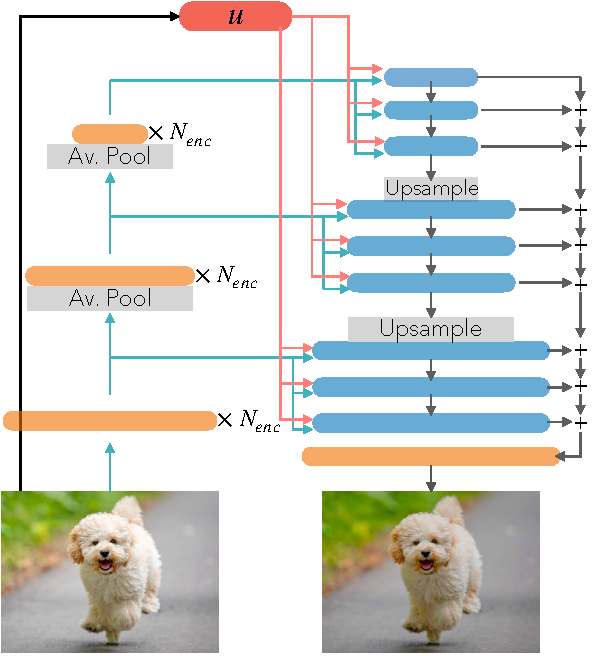
\includegraphics[width=0.51\linewidth]{pics/5_dvp/_full_model.pdf}}}
    &      
    \adjustbox{valign=b}{
        \begin{tabular}{@{}cc@{}}
        \multicolumn{2}{c}{
            \subfloat[Top down block\label{subfig:top_down}]{%
                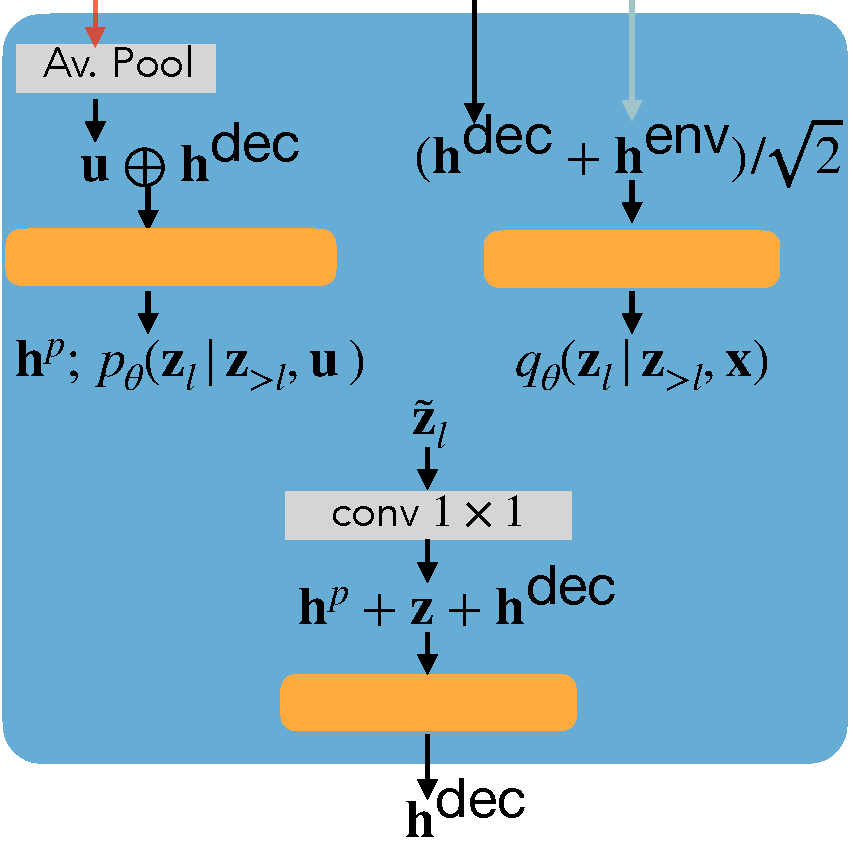
\includegraphics[width=.28\linewidth]{pics/5_dvp/_top_down_dct_2.pdf}}
        }\\
            \subfloat[Resnet block\label{subfig:resnet}]{%
                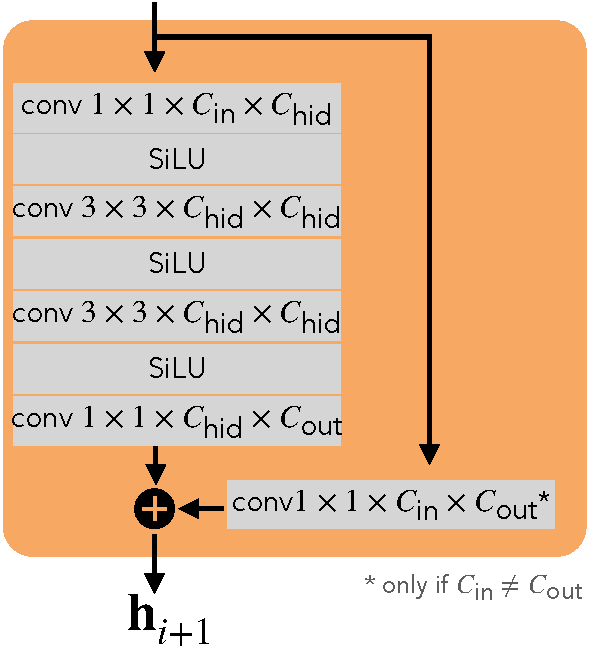
\includegraphics[width=.25\linewidth]{pics/5_dvp/_resnet_block.pdf}} &
            \subfloat[Pseudoinput block\label{subfig:context}]{%
                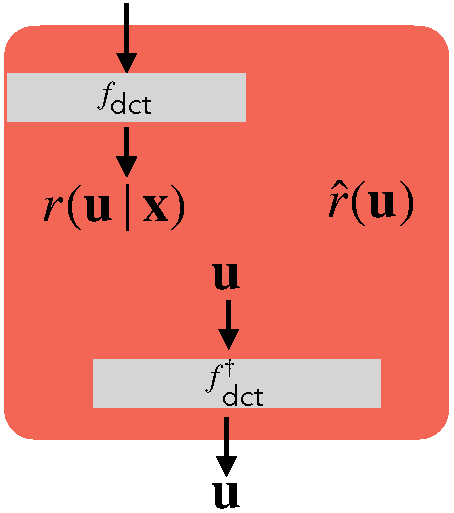
\includegraphics[width=.25\linewidth]{pics/5_dvp/_context_block.pdf}} \\
    \end{tabular}}
    \end{tabular}
    }
    % \caption[][\baselineskip]{A diagram of the DVP-VAE: TopDown hierarchical VAE with the diffusion-based VampPrior.\\
    %  (a) A \textit{BottomUp} path (left) and a \textit{TopDown} path (right). (b) A \textit{TopDown} block that takes features from the block above $\mathbf{h}^{dec}$, encoder features $\mathbf{h}^{enc}$ (only during training) and a pseudoinput $\rvu$ as inputs. (c) A single Resnet block. (d) A single pseudoinput block.
    % } 
    \captionsetup{width=1.3\textwidth, margin={0pt, -.3\textwidth}}
    \caption{A diagram of the DVP-VAE: TopDown hierarchical VAE with the diffusion-based VampPrior.
     (a) A \textit{BottomUp} path (left) and a \textit{TopDown} path (right). (b) A \textit{TopDown} block that takes features from the block above $\mathbf{h}^{dec}$, encoder features $\mathbf{h}^{enc}$ (only during training) and a pseudoinput $\rvu$ as inputs. (c) A single Resnet block. (d) A single pseudoinput block.
    } 
    \label{fig:model_schema}
    % \vskip 15pt
    \vskip -15pt
  \end{figure*}
  
The model architecture and parameterization are crucial to the scalability of the model. In this section, we discuss the specific choices we made.
The starting point for our architecture is the architecture proposed in VDVAE~\citep{Child2020-ze}. However, there are certain differences. We schematically depict our architecture in Figure~\ref{fig:model_schema}. We consider a hierarchical TopDown VAE with $L$ stochastic layers, namely, latent variables $\rvz_1, \dots, \rvz_L$. We assume that each latent variable has the same number of channels, but they differ in spatial dimensions: $\rvz_l \in \mathbb{R}^{c \times h_l \times w_l}$. We refer to different spatial dimensions of the latent space as \textit{scales}.

 \subsection{Bottom-up} \label{subsec:arch_encoder}
The bottom-up part corresponds to calculations of intermediary variables dependent on $\rvx$. We follow the implementation of \citet{Child2020-ze} for it. We start from the bottom-up path depicted in Figure~\ref{fig:model_schema}a (left), which is fully deterministic and consists of several ResNet blocks (see Figure~\ref{fig:model_schema}c)\citep{he2016deep}. 
The input is processed by $N_{\text{enc}}$ blocks at each scale, and the output of the last resnet block of each scale is passed to the TopDown path in Figure~\ref{fig:model_schema}a (right). Note that here $N_{\text{enc}}$ is a separate hyperparameter that does not depend on the number of stochastic layers $L$.
  

 \subsection{TopDown} \label{subsec:arch_decode}
The TopDown path depicted in Figure~\ref{fig:model_schema}a (right) computes the parameters of the variational posterior and the prior distribution starting from the top latent variable $\rvz_L$. 

The first step is the pseudoinput block shown in Figure~\ref{fig:model_schema}d. Using the deterministic function $f_{\text{dct}}$, it creates the pseudoinput random variable from the input $\rvx$ (see Algorithm~\ref{alg:context_forward}) that is used to train the Diffusion-based VampPrior $\hat{r}_{\gamma}(\rvu)$.
At test time, a pseudoinput is sampled using this unconditional prior. The pseudoinput sample is then converted back to the input domain (see Algorithm~\ref{alg:context_backward}) and used to condition prior distributions at all levels $p_{\theta}(\rvz_{1:L}|\rvu)$.

Next, the model has $L$ TopDown blocks depicted in Figure~\ref{fig:model_schema}b. 
Each TopDown block takes deterministic features from the corresponding scale of the bottom-up path denoted as $h_{\text{enc}}$, the output of the pseudoinput block $\rvu$, and deterministic features from the TopDown block above $h_{\text{dec}}$ as inputs. Our implementation of this block is similar to the VDVAE architecture, but there are several differences that we summarize below:
\begin{itemize}%[leftmargin=*]
    \item \textit{Incorporating pseudoinputs}\\
    We concatenate the pseudoinput (properly reshaped using average pooling) with $h_{\text{dec}}$ to compute the parameters of the prior distribution. 
    \item \textit{Variational posterior parameters} \\
    We assume that both $h_{\text{dec}}$ and $h_{\text{enc}}$ have the same number of channels, allowing us to sum them instead of concatenating. This reduces the total number of parameters and the memory consumption.
    \item \textit{Additional ResNet Connections}\\
    Our TopDown block has three ResNet blocks (Figure~\ref{fig:model_schema}c). In contrast to our architecture, in VDVAE only the block that updates $h_{\text{dec}}$ has a residual connection. 
\end{itemize}

We did not observe any training instabilities and did not apply the \textit{gradient skipping} used in \citet{Child2020-ze}.

 \subsection{Latent Aggregation in Conditional Likelihood} \label{subsec:latent_aggr}

% \paragraph{Latent Aggregation}
The last important element of our architecture is the \textit{aggregation of latents}. Let us denote samples from either the variational posteriors $q_{\phi}(\rvz_{1:L}|\rvx)$ during training or the prior $p_{\theta}(\rvz_{1:L}|\rvu)$ during generating new data as $\tilde{\rvz}_1, \dots, \tilde{\rvz}_L$.  
Furthermore, let $\vh_1$ be the output of the last TopDown block. 
These deterministic features are computed as a function of all samples $\tilde{\rvz}_1, \dots, \tilde{\rvz}_L$.
Therefore, it can be used to calculate the final likelihood value.
% \begin{align}\label{eq:cond_like_vdvae}
%     p_{\theta}(\rvx | \rvz_{1:L}) = p_{\theta}(\rvx | \text{Conv}(\vh_1)).
% \end{align}
However, we observe empirically that in such parameterization some layers of latent variables tend to be completely ignored by the model.
Instead, we propose to enforce a strong connection between the conditional likelihood and all latent variables by explicitly conditioning on all of the sampled latent variables, namely: 
\begin{align} \label{eq:cond_like_ours}
    p_{\theta}(\rvx | \rvz_{1:L}) = p_{\theta}\big( \rvx \big| \text{NN}\big(\frac{1}{\sqrt{L}}\sum\nolimits_l \tilde{\rvz}_l\big) \big).
\end{align}

We refer to this as the \textit{latent aggregation}.
We show empirically in the experimental section that this leads to a consistently high ratio of active units. 

 % \begin{table}
 %    % \begin{minipage}[c]{0.65\textwidth}
 %        \centering
 %        \caption{Differences between Very Deep VAE and DCT-VAE
 %        }
 %        \label{tab:main_results}
 %        \begin{tabular}{l| cc}
 %            \toprule
 %              & VDVAE & Ours\\
 %            \midrule
 %           Activation function & \\
 %            % Optimizer \\
 %            ResNet connections \\
 %            q\_net  \\
 %            Upsampling \\
 %            \bottomrule
 %        \end{tabular}% % \end{varwidth}%\hfill 
 % \end{table} 



